\chapter{{Introduction}}
\label{chap:introduction}
\minitoc

\thispagestyle{empty}

\newpage
%%%%%%%%%%%%%%%%%%%%%%%%%%%%%%%%%%%%%%%%%%%%%%%%%%%%%%%%%%%%%%%%%%%%%%%%%%%%%%
Modelling, analysis and control of mechanical systems with impacts is an interesting and open problem which attracts the attention of a wide range of researchers, from physicists and mechanical engineers to specialists in control and automation~\cite{brogliato1999nonsmooth,stronge2018impact}.
The interaction between continuous and discrete-time dynamics arises, for instance, while considering the behavior of a mechanical system in presence of impacts, as its dynamics cannot be represented only by means of differential equations. The theory of~\textit{hybrid dynamical systems} (HDS) is the formalism used to accurately describe this peculiar phenomena. Overviews of this framework are given by~\cite{van2000introduction,haddad2006impulsive}. In particular, the most general modeling approach is the one of \textit{hybrid inclusions} developed in recent years \cite{goebel2009hybrid}.

When dealing with modelling and control of physical systems, one of the most popular state--of--the--art approaches is the the \textit{port-Hamiltonian} (PH) theory \cite{secchi2007control,van2014port}. PH systems provide a framework which can be employed to model physical systems from an energetic point of view, explicitly capturing the phenomena of energy storage, energy dissipation and energy routing. 

\section{Motivation}
% %
% \subsection{Nonprehensile Manipulation}
% %
%The main purpose of this thesis is to provide a novel general and unified framework to model and control highly dynamic robotic tasks from an energetic point of view. However, the generality of the developed framework allows to go bey 
%%%%%%%%%%%%%%%%%%%%%%%%%%%%%%%%%%%%%%%%%%%%%%%%
\subsection{The Manipulation Problem for Highly Dynamic Tasks}
\subsection{The Role of Energy in Robot Control}
In the last three decades, the fundamental concept of \textit{energy} experienced an impressive growth process in engineering practice and in particular in system theory. 
%
\newline

%
The framework of \textit{passivity--based control} (PBC) is now a well--established branch in nonlinear control theory and aims at treating dynamical systems as devices able to exchange energy, rather than to process signals \cite{ortega2001putting}. 
This is possible by equipping dynamical systems with additional structure (e.g. storage functions, supply rates, etc.) by means of which the concepts of energy and input/output characterisation of the system are connected in a unique framework \cite{sontag2008input}.
%
\newline

%
The other fundamental aspect of this paradigm is \textit{interconnection} of systems by means of \textit{power ports} \cite{duindam2009modeling}, which led to the definition of \textit{port-Hamiltonian systems} \cite{ortega2001putting,MASCHKE1992359,van2014port}, the mathematical framework in which PBC developed naturally, merging geometry and network theory. Hence, the control problem reduces to the design of a dynamical system (the controller) and an interconnectionstructure that ``shapes'', in a desired way, the energy of the original system \cite{ortega2001putting,ortega2008control}.
%
\newline

%
This approach allows control engineers to pay particular attention to the performance of the control system and not only to stabilizability (as common in nonlinear control).
%
\newline

%
In classic robot control, the theory of passivity lead to several successful approached, such as the \textit{gravity--compensation} \cite{arimoto1984stability} and \textit{impedance} controller. Other interesting application are robots with flexible links \cite{macchelli2009} and elastic joints \cite{zhang2016}.
%
%%%%%%%%%%%%%%%%%%%%%%%%%%%%%%%%%%%%%%%%%%%%%%%%%%%%%%%
\subsection{Energy as Common Factor Among Interactions}
%
Driven by a physical intuition, it is rather straightforward recognizing energy as the \textit{lingua franca} between different physical domains. This idea lead, in the early sixties, Paynter to start the field of \textit{port--based modeling} \cite{paynter1961analysis}.
%
\newline

%
A physical system, in fact, may exhibit a \textit{dynamical behavior} if and only if some energy exchange happen within its \textit{internal structure} (components) or with the external world. In any phisycal domain there exists pair of dual variables (see...) often called \textit{flows} and \textit{efforts} which intrinsically form \textit{power ports}, interfaces through which energy flows \cite{secchi2007control}. Table \ref{tab:ef} lists the effort and flow variables for several physical domains.
%
\begin{table}[b]
	\centering
	\begin{tabular}{|c|cc|cc|} \hline
			\rowcolor{gray!50}\textbf{Domain}&{\centering \textbf{Effort}}&&{\centering \textbf{Flow}}&\\\hline
			Mechanics (translational)&Force&$F$&Velocity&$v$\\\hline
			\rowcolor{gray!15}Mechanics (rotational)&Torque &$\tau$&Angular Velocity &$\omega$\\\hline
			Electric&Voltage &$v$&Current &$i$\\\hline
			\rowcolor{gray!15}Hydraulic&Pressure& $p$&Volume Flow &$Q$\\\hline
			Thermodynamical&Temperature &$T$&Entropy Flow &$\dot{E}$\\\hline
	\end{tabular}
	\caption{Efforts and flows variables for various physical domains}
	\label{tab:ef}
\end{table}
%
\newline

In the context of robot manipulation, this description of dynamical phenomena may result particularly useful to model the interaction between the robot end--effector and the object, which indeed exchange energy with each other in a continuous fashion.
%
In fact, the port--Hamiltonian framework allows to explicitly capturing the physical phenomena behind this continous interaction. Furthermore, in this perspective, the robot controller can also be thought as an other dynamical system interconnected with the robot exchanging energy with it. 
This approach results to be both, general and versatile.
%
The theory of passivity--based control of port--Hamiltonian system has been already successfully applied in a variety of manipulation tasks: from grasping \cite{stramigioli99} and soft--finger manipulation \cite{ficuciello2010} to non--prehensile tasks, e.g. object rolling \cite{donaire2017,serra2019}.
%
\newline

%
Besides, when the robot tasks involve \textit{nonsmooth} phenomena such as mechanical impacts or dynamic friction \cite{brogliato1999nonsmooth}, the state--of--the--art passivity--based techniques cease to work due to the discontinuities in system's state along trajectories. 
Therefore, it would be desirable to extend the theory to the hybrid case. In fact, if this can be achieved, a new general and unified framework to model and control robots highly dynamic tasks would be established.
%
\newline

Examples of these tasks in the manipulation context are:
ball--juggling \cite{sanfelice2007hybrid, tian2013}, ball--dribbling \cite{Batz2010, haddadin2018exploiting}, \cite{ruggero2018}
%
%%%%%%%%%%%%%%%%%%%%%%%%%%%%%%%%%%%%%%%%%%%%%%%%%%%%%%%%%%%%%%%%%%%%%
\subsection{Hybrid port--Hamiltonian System: a New Tool For Robotics}
%

%
%%%%%%%%%%%%%%%%%%%%%%%%%%%%%%%%%
\subsection{Beyond Robot Control}
Up to this point we discussed the need of an hybrid framework in robotics due to the \textit{nonsmooth} nature of several crucial robot tasks.
However, in many situations, it is the controller itself to be hybrid in nature. In example, the temperature regulator of a room or the motion controller of a soccer playing humanoid robot. 
Therefore, the theory

%%%%%%%%%%%%%%%%%%%%%%%%%%%%%%%%%%%%%%%
\subsection{The Identification problem}

\begin{figure}
    \centering
    \def\firstcircle{(0,0) circle (2.5cm)}
    \def\secondcircle{(45:3.5cm) circle (2.5cm)}
    \def\thirdcircle{(0:4.5cm) circle (2.5cm)}
    \def\id{(3,-2.5) ellipse (0.65 and 0.65)}
    \def\hds{(3,-1.3) ellipse (1.5 and 1.2)}
    \def\ph{(3.2,0) ellipse (1.5 and 1.2)}
    \definecolor{carminered}{rgb}{1.0, 0.0, 0.22}
    \definecolor{cerulean}{rgb}{0.0, 0.48, 0.65}
    \definecolor{bluegray}{rgb}{0.4, 0.6, 0.8}
    \definecolor{amber}{rgb}{1.0, 0.75, 0.0}
    \definecolor{emerald}{rgb}{0.31, 0.78, 0.47}
    %
    \begin{tikzpicture}
        \draw[thick, fill=gray!30,fill opacity=0.3] \firstcircle;
        \draw[thick, fill=gray!30,fill opacity=0.3] \secondcircle node [above] {};%{\small Control Theory};
        \draw[thick, fill=gray!30,fill opacity=0.3] \thirdcircle node [below] {};%{Statistics};
        \draw[thick, fill=gray!50,fill opacity=0.4, rotate = 60] \hds node [below] {};%{Statistics};
        \draw[thick, fill=gray!50,fill opacity=0.4, rotate = 60] \ph node [below] {};%{Statistics};
        \draw[thick, fill=gray!50,fill opacity=0.4, rotate = 60] \id node [below] {};%{Statistics};
        %
        \begin{scope}[rotate = 60]
            \clip \hds;
            \draw[thick, fill = amber] \ph;
        \end{scope}
        %
        \begin{scope}[rotate = 60]
            \clip \hds;
            \clip \firstcircle;
            \draw[-,black,thick, fill = bluegray] \ph;
        \end{scope}
        %
        \begin{scope}[rotate = 60]
            \clip \hds;
            \fill[emerald] \id;
        \end{scope}
        %%%%%%%%%%%%
        \draw (0,0)   node[]{\textbf{Robotics}};
        \draw (0:4.5) node[]{\textbf{Statistics}};
        \draw (2.55,4.45) node[]{\textbf{Control Theory}};
        \draw (-1,4.75) node[] (ph) {Port--Hamiltonian Systems};
        \draw (7.25,3.25) node[] (hds) {Hybrid Dynamical Systems};
        \draw (8,2) node[] (id) {System Identification};
        %
        \draw[-o, thick] (ph.south) to[out = -90,in = 150] (1.5,3);
        \draw[-o, thick] (hds.south) to[out = -90,in = 50] (3.5,2.5);
        \draw[-o, thick] (id.south) to[out = -90,in = -50] (3.85,1.25);
        %%%
        \draw (-1,-3) node[] (ch4) {\color{amber}\textbf{Chapter 4}};
        \draw (3,-3) node[] (ch5) {\color{bluegray}\textbf{Chapter 5}};
        \draw (7,-3) node[] (ch6) {\color{emerald}\textbf{Chapter 6}};
        %
        \draw[-o, dashed, thick] (ch4.north) to[out = 45,in = 180, distance = 4cm] (2.35,2.5);
        \draw[-o, dashed, thick] (ch5.north) to[out = 110,in = 250] (1.6,1.75);
        \draw[-o, dashed, thick] (ch6.north) to[out = 120,in = 250, distance = 3cm] (3.4,1.5);
    \end{tikzpicture}
    \caption{Caption}
    \label{fig:my_label}
\end{figure}
\clearpage
%%%%%%%%%%%%%%%%%%%%%%%%%%%%%%%%%%%%%%%%%%%%%%%%%%%%%%%%%%%%%%%%%%%%%%%%%%%%%%%

\section{{Objective and Approach}}
The aim of this thesis is to present a novel control theoretical framework for physical systems with nonsmooth and multimodal behaviors, with a special insight toward robot control tasks where the current--state--of--the--art approaches fail.

The main objectives are:
%
\begin{itemize}
    \item [1.] \textbf{to develop a novel control theoretical framework merging the theories of port--Hamiltonian systems and hybrid systems}.
    
    Driven by the aim of solving a robot control problem, the theory of \textit{hybrid port--Hamiltonian systems} is developed from the theory of port--Hamiltonian systems and \textit{hybrid inclusions}, one of the most general representations of hybrid dynamical systems.
    %
    \item [2.] \textbf{to apply the developed theory to a robot control task to prove its effective within the robotics framework}. 
    
    Considering the ball--dribbling robot problem, a novel controller, the \textit{iterative energy shaping} is systematically synthesized, proving the the capabilities of the proposed framework.
    %
    \item [3.] \textbf{to show how the developed theory goes beyond robotics and can be used to model a broad variety of control systems}. 
    
    The problem of controlling a linear time--invariant system with countable set points is considered. At first, a nonlinear passive controller is used to stabilize simultaneously all the set points. Then, a hybrid optimal impulse controller is designed to switch the between the set points. Finally, it is shown how the controlled system can be modeled as hybrid port--Hamiltonian system, implicitly inheriting some useful properties to analyze its behaviour.
    
    \item[4.] \textbf{to derive a new systematic identification procedure for a class of hybrid systems}.
    
    As most of hybrid control systems (including the proposed ones) require some knowledge of the physical parameters of the controlled plant, a new systematic procedure is presented to solve the estimation problem. It is shown how this method can be applied to a variety of hybrid port--Hamiltonian systems 
    
    \end{itemize}
%





%
\clearpage
%%%%%%%%%%%%%%%%%%%%%%%%%%%%%%%%%%%%%%%%%%%%%%%%%%%%%%%%%%%%%%%%%%%%%%%%%%%%%%%

%\section{Problem Setting}
% In this thesis the problem addressed is to build a glass confidence map mentioned above by a mobile robot automatically using a LRF, specifically in human indoor environments where large areas of glass panels exist, such as shopping malls, and offices. Several assumptions are made in this thesis. The first assumption is the LRF is mounted on the mobile robot and scans the environment horizontally. The LRF outputs both distance to the objects and received reflected laser intensity, which is true for most LRFs on market. Second, the robot's motion is considered to be planar, and it's odometry information is assumed to be readily available from the robot's sensors, such as encoders. Reasonable noise is allowed for the odometry information. Third, the glass as well as other main objects in the environments are assumed to be not curved. Curve surface cannot be handled in current work but is possible to be solved by some improvements. However, there is no assumption regarding the cleanness, thickness or color of the glass panels as well as other objects. 

% To use the proposed method to build glass confidence maps, the classifier needs to be trained using previously acquired experimental data. Once the classifier is trained, it can work on same module of LRFs and similar environments. "Similar environments" means the material types are similar with the ones in the training environments but do not need to be exact same. More details about the extensibility and robustness of the classifier when dealing with untrained materials will be discussed in Chapter 5. Moreover, while building the map, a mobile robot needs to be tele-operated to navigate in the environment, with the mapping system running on the robot. Simultaneously, a standard SLAM algorithm should be running in order to provide a 2-D glass confidence map of the environment and the robot's location on the fly. 

%\clearpage
%%%%%%%%%%%%%%%%%%%%%%%%%%%%%%%%%%%%%%%%%%%%%%%%%%%%%%%%%%%%%%%%%%%%%%%%%%%%%%%

\section{Thesis Contenent \& Structure}
This thesis is structured in seven chapters as follows: this chapter serves as an introduction that describes the main motivations, purpose and approach of this study.
These seven chapter can be logically clustered in four main parts: Introduction and backgroud, theoretical results, applications and conclusions  
%
\newline

%
\textbf{Chapter 2} briefly introduces the fields of port--Hamiltonian systems and hybrid dynamical systems. Throughout the chapter, several illustrative examples related to robotics, mathematical biology and physics will be provided to highlight the practical importance of the presented theoretical concepts. 

In the first half of the chapter, the input--state--output model of a port-Hamiltonian system is derived and its most relevant properties are enounced. Moreover, the basic theory of the energy--balancing passivity--based control is also recalled. In the second part of the chapter, the basic results on hybrid systems are introduced. In particular, it will be focused on the class of \textit{hybrid inclusions} and its stability/passivity theory.  The chapter concludes with a summary of the previous attempts to merge the two frameworks and their main limitations. 
%
\newline

%
\textbf{Chapter 3} deals with the definition and characterization of hybrid-port Hamiltonian systems. Starting from the concepts revised in the previous chapter, the new framework is here consistently developed. First, the basic assumptions are stated and the hybrid port--Hamiltonian model is derived. The concept of passivity is subsequently extended to the new model. Necessary and sufficient conditions for passivity are also reported and proved. Then, Lyapunov stability is extended from the one for hybrid inclusions. Finally, all the previous results are used to transfer to the hybrid case some of the features of passivity--based control for port--Hamiltonian systems. As for Chapter 2, application examples will be provided throughout the chapter.
%
\newline

%
\textbf{Chapter 4} introduces the first real application of the developed theory. In particular, the problem of modelling and control a ball--dribbling robot is considered. The main challenges offered by this systems are: underactuation, dynamic decoupling between the robot and the ball, impacting interactions. First, the system is consistently modeled in hybrid port--Hamiltonian form. Then, a novel energy--based controller is derived from physical intuitions on the system. This controller enhance the classic energy shaping with the iterative learning, allowing the robot to rhythmically bounce the ball at a desired height. Simulations are performed to prove the effectiveness and robustness of the controller.   
%
\newline

%
\textbf{Chapter 5}  %
\newline

%
\textbf{Chapter 6} introduces the first real application of the developed theory. Although sever physical example are provided in the previous chapters. %
\newline

%
\textbf{Chapter 7} presents the conclusions of this study and future work. An outline of the whole thesis structure is shown in Fig. \ref{fig:ThesisStructure}.

\begin{figure}[b]
    \centering
    \definecolor{darkspringgreen}{rgb}{0.09, 0.45, 0.27}
    \tikzstyle{container} = [rectangle, draw, semithick, rounded corners,
                     text width=44mm, minimum height=11mm, align=center,
                     fill=white, drop shadow, inner sep=0.6cm]
    \begin{tikzpicture}[
        node distance = 5mm and 4mm,
        %every node/.style = {font=\bfseries\itshape},
        chapter/.style = {rectangle, draw, semithick, rounded corners,
                     text width=44mm, minimum height=9mm, align=center,
                     fill=white, drop shadow},  
                     ys/.style = {yshift=-5mm}         
                    ]
        \draw[thick] (0,0)  coordinate (A1)
                    node[below right] {Preliminaries \& Background} 
                    -- + (\textwidth,0)
                    coordinate (B1);
        \node (ch1) [chapter, below=of $(A1)!0.5!(B1)$]         {\textbf{Chapter 1}\\ \textit{Introduction}};
        \node (ch2a) [chapter, below  left=1.5cm and -2cm of ch1] {Port--Hamiltonian Systems};
        \node (ch2b) [chapter, below right=1.5cm and -2cm of ch1] {Hybrid Dynamical Systems};
        \node [container,fit=(ch2a) (ch2b), yshift = 0.5cm] (c1) {\textbf{Chapter 2}\\ \textit{Preliminaries}\textcolor{white}{\\aa\\aa}};
        \node (ch2a) [chapter, below  left=1.5cm and -2cm of ch1] {Port--Hamiltonian Systems};
        \node (ch2b) [chapter, below right=1.5cm and -2cm of ch1] {Hybrid Dynamical Systems};
        %
        \draw[thick] ([ys] A1 |- ch2a.south)  coordinate (A2)
                    node[below right] {Theoretical Results}
                    -- + (\textwidth,0)
                    coordinate (B2);
        \node (ch3) [chapter, below=of $(A2)!0.5!(B2)$,text width=54mm, fill = gray!50]   {\textbf{Chapter 3}\\\textit{Hybrid Port--Hamiltonian Systems}};
        %\node (ch3) [chapter, below  left=of $(A2)!0.5!(B2)$]   {State of the Art};
        %\node (ch4) [chapter, below right=of $(A2)!0.5!(B2)$]   {Building of Theory};
        \draw[thick] ([ys] A1 |- ch3.south)  coordinate (A3)
                    node[below right] {Applications}
                    -- + (\textwidth,0)
                    coordinate (B3);
        \node (ch4) [chapter, below=of $(A3)!0.5!(B3)$,text width=84mm, fill = gray!50] {\textbf{Chapter 4}\\\textit{Iterative Energy shaping of a Ball--dribbling Robot}};
        \node (ch5) [chapter, below=of ch4,text width=84mm, fill = gray!50]                     {\textbf{Chapter 5}\\\textit{Multistable Energy Shaping with Hybrid Mode Selector}};
        \node (ch6) [chapter, below=of ch5,text width=84mm, fill = gray!50]                     {\textbf{Chapter 6}\\\textit{Identification of a Class of Hybrid Systems}};
        \draw[thick] ([ys] A1 |- ch6.south)  coordinate (A4)
                    node[below right] {Conclusion}
                    -- + (\textwidth,0)
                    coordinate (B4);
        \node (ch7) [chapter, below=of $(A4)!0.5!(B4)$]         {\textbf{Chapter 7}\\Discussion and conclusions};
        %\node (ap1) [chapter, below  left=of ch7]               {\textbf{Appendix A}};
        %\node (ap2) [chapter, below =of ch7]                    {\textbf{Appendix B}};
        %\node (ap3) [chapter, below right=of ch7]               {\textbf{Appendix C}};
        %
        \draw [-latex, ultra thick, blue] (ch1)--(c1);
        \draw [-latex, ultra thick, blue] (ch2a.south) to[out=-45,in=90] (ch3.north);
        \draw [-latex, ultra thick, blue] (ch2b.south) to[out=-135,in=90] (ch3.north);
        \draw [-latex, ultra thick, blue] (ch3.south) to[out=-90, in=90] (ch4.north);
        \draw [-latex, ultra thick, blue] (ch3.south) to[out=-155,in=130,distance=3.5cm] (ch5.west);
        \draw [-latex, ultra thick, red] (ch2b.south) to[out=-45,in=30,distance=2.5cm] (ch6.east);
        \draw [-latex, ultra thick, darkspringgreen] (ch6.south)--(ch7.north);
        \draw [-latex, ultra thick, darkspringgreen] (ch5.west) to[out=200,in=180,distance=1.5cm] (ch7.west);
        \draw [-latex, ultra thick, darkspringgreen] (ch4.west) to[out=200,in=180,distance=3cm] (ch7.west);
    \end{tikzpicture}
    \vspace{5mm}
    \caption{Thesis structure outline. The coloured arrows indicate the logical flows of the contents throughout the thesis, highlighting, e.g., how the theory presented in the first chapters is employed in the various applications. Chapters in light gray blocks contain exclusively original content developed by the author,}
    \label{fig:ThesisStructure}
\end{figure}
\clearpage
%%%%%%%%%%%%%%%%%%%%%%%%%%%%%%%%%%%%%%%%%%%%%%%%%%%%%%%%%%%%%%%%%%%%%%%%%%%%%%%
\iffalse
A major challenge in robotics is to free robots from controlled industrial settings and allow them to interact with humans and dynamic environments. Biologically inspired modelling could be used to create more robust system which try to mimic nature and help to address this challenge. Complex tasks that require dexterous in-hand manipulation, which are effortless for humans, have been proved to be extremely complicated for robots. In fact, they require a deep knowledge of object’s dynamics. This open issue has been approached by many researchers. When the robot manipulation tasks involve higher dynamic, e.g. bouncing, throwing and catching a ball, control design becomes even more complex in in these scenarios mechanical impacts are involved and inevitably determine discontinuities in the system’s states. In this setup, classic techniques can no longer be employed, and current literature only addresses the problem for specific tasks [1]. Indeed, a unified framework is still missing. For this reason, during my Master course at the University of Tokyo I started to develop a novel unified framework to model and control interactive robotic systems in which dynamic interaction do not allow the application of standard control techniques. The idea behind my main results is the one of recognizing energy as lingua franca among different types of interactions [1]: when a robot is touching an object, it is indeed exchanging energy with it; moreover, when the robot hits the object, causing a sudden change in its velocity, an energy flow between the bodies occurs. Following this argument, we developed the framework of hybrid port-Hamiltonian systems (HPHs) merging the most promising theories related to robot control. Simple simulative experiments on a challenging, but ubiquitous, ball-dribbler robot show the validity and robustness of the proposed approach. However, no experimental tests have yet been completed. We also submitted a paper to WROCO ’19 (IFAC).
(1) Research Objective: 
The main research objective during my PhD will be the one of experimentally demonstrating the effectiveness of the new theoretical framework, by solving practical robot tasks, e.g. non prehensile manipulation tasks. In the first place, I would like to focus on the ball-dribbling robot problem, then the ball throwing/catching and other tasks. To do this I will encounter several challenges, particularly from the implementation point of view.
(2) Research Plan: what and how 
Before my master’s graduation I will complete the development of the control theoretical framework and submit the results to the Transactions on Automatic Controls. Then, my PhD research activity will be methodologically divided in three phases that will span over three years: mathematical modeling, hardware and software development, experimental evaluation and data analysis.
(3) Collaborations: 
I am planning to collaborate with a researcher from the Robotics departement of Univeristy of Twente (NL) on the theoretical part. Regarding the implementation (in particular the calibration part) I will be aided by a mechanical engineer of ETH Zurich. I will also continue, as side research, to collaborate with Prof. Jinkyoo Park of KAIST.
(4) Abroad research period: 
During the second year of my PhD am planning to spend three to six month in a foreign university, cointinuing there the same research projet. Most likely ETH Zurich, in the laboratory led by Roland Siegwart, since they work on similar robot tasks as mine, or UCSB with Prof. Ricardo Sanfelice who works in the field of hybrid systems and could aid me solving some of the theoretical issues.
(1) Research Features, Key Focuses, and Innovative Aspects: The HPHs framework merges the theories of hybrid dynamical systems (HDs) with the one of port-Hamiltonian systems (PHs). Hybrid systems allow to The key innovative aspect of the proposed control approach is that the energy-based modeling allows a fine tuning of the robot task performances. This property is groundbreaking in robot control as classic techniques only focus on stabilization and not on performance. With respect to standard modeling methods, the HPHs offer a holistic perspective to the control problem, where particular focus is given to the robot’s interactions from an energy exchange point of view. 
(2) Research position and significance in related researches in Japan and abroad: HDs are recently gaining interest among the scientific community. Notable researchers are 合原 一幸 (東京大学), Andrew Teel (UCSB) Ricardo Sanfelice (UCSC). Similarly, both in Japan and in the world, PHs are now an affirmed research field. In particular, world-class Japanese scientists of the topic are井村 順一 (東京工業大学) and 藤本 健治 (京都大学). Other main developer of PHs theory resides in Netherland and France. Researches related to these fields, however, are more theoretical than practical. I had the pleasure to speak several times with Prof. Stefano Stramigioli of University of Twente and I always had a great feedback from him. My topic could really become the melting pot of several theories which can finally find a practical application for cutting-edge technology.
(3) Research expected impacts and future prospects: My research will hopefully result in more precise and robust robot control algorithms. In practical situation, systems are always affected by errors (sensing, actuation) which must be taken into account for a reliable and safe human-robot interaction. This is one of the biggest limits in the employment of robot technology in social contexts. Toyota, in example, should deploy robots across the Tokyo 2020 Olympic sites to aid workers and attendees. Robots equipped with our novel control method will be capable of smoother, “human-like”, movements while taking into account safety issue. As direct consequence of our research work, robots’ capabilities to interact with their environments would grow and so would their ability to be of good use to our society.

{\color{red}
\subsection{WROCO19}
Modelling, analysis and control of mechanical systems with impacts is an interesting and open problem which attracts the attention of a wide range of researchers, from physicists and mechanical engineers to specialists in control and automation~\cite{brogliato1999nonsmooth,stronge2018impact}.
The interaction between continuous and discrete-time dynamics arises, for instance, while considering the behavior of a mechanical system in presence of impacts, as its dynamics cannot be represented only by means of differential equations. The theory of~\textit{hybrid dynamical systems} (HDS) is the formalism used to accurately describe this peculiar phenomena. Overviews of this framework are given by~\cite{van2000introduction,haddad2006impulsive}. In particular, the most general modeling approach is the one of \textit{hybrid inclusions} developed in recent years \cite{goebel2009hybrid}.

When dealing with modelling and control of physical systems, one of the most popular state--of--the--art approaches is the the \textit{port-Hamiltonian} (PH) theory \cite{secchi2007control,van2014port}. PH systems provide a framework which can be employed to model physical systems from an energetic point of view, explicitly capturing the phenomena of energy storage, energy dissipation and energy routing. 
%This approach results to be both, general and versatile, since energy can be considered as a common factor between different physical domains. A description of the finite--dimensional port-Hamiltonian systems is presented in \cite{secchi2007control,van2014port}.
%This formalism might be particularly useful in the analysis and study of complex systems, which can be considered as a network of simpler subsystems that, upon interconnection, combine their energy properties to determine the behavior of the full system~\cite{915398}.
%The PH approach plays also leading role in the modeling and control of infinite--dimensional systems \cite{MASCHKE200027,macchelli2004port,macchelli2004port2,8263926,MACCHELLI201854}.
In this perspective a controller can also be thought as a dynamical system interconnected with the plant and exchanging energy with it. 
%The control problem might be then reformulated as: finding a dynamical system and an interconnection pattern such that the overall energy function of the system reaches the desired ``shape".
This idea led to the definition of \textit{energy shaping} \cite{ortega2001putting}, which represent a fruitful application of passivity-based control (PBC).
% As passivity plays a fundamental role in modern nonlinear control theory, it is also gaining popularity in the HDS framework, e.g. \cite{spong2007passivity,carrasco2010passivity}. In particular, the definition of passivity for hybrid inclusions has been introduced in \cite{naldi2011passivity,naldi2013passivity}.

% Some attempts have been done to merge the theories of PH systems and HDS for both modeling \cite{valentin2006hybrid,valentin2007port} and control \cite{haddad2003energy,5400785}. More specifically, in \cite{valentin2006hybrid,valentin2007port,5400785} physical switching systems are modelled in an \textit{implicit} PH fashion by employing network graph theory and geometric constraints on the interconnection structure. 
%The derived framework can be used in main practical application for switching electrical circuits.
%A state transfer principle for switching port-Hamiltonian systems was also proposed in~\cite{5400785}. The derived system, which is an exstension of the charge/flux conservation principle to RLC circuits, was successfully used to swithing a mechanical system. 
%Regarding the control design problem, an energy--based method for a class of (mechanical) impulsive PH systems has been addressed in \cite{haddad2003energy}.

In this paper we present a novel method for controlling a \textit{ball--dribbling} robot.
A representation of the system is given in Figure \ref{fig:1D}.
\begin{figure}[!t]
	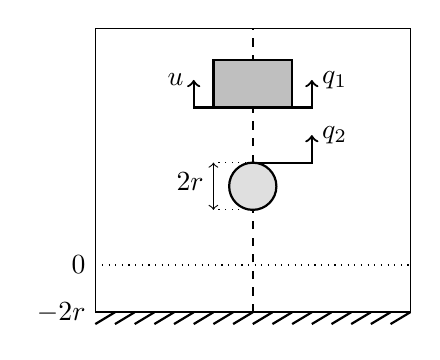
\begin{tikzpicture}
	%
	% axes
	\draw[thick] (0,-0.6)--(4,-0.6);
	%\draw[thick,dashed,red!40] (0,0) node[anchor = east] {\color{black}$0$}--(4,0);
	\draw[dotted] (0,0) node[anchor = east] {\color{black}$0$}--(4,0);
	\draw[thick,dashed] (2,-0.6) -- (2,3);
	\draw (0,-0.6) node[anchor = east] {$-2r$} -- (4,-0.6) -- (4,3) -- (0,3) -- (0,-0.6);
	
	% robot
	\fill[gray!50, draw = black,thick] (1.5,2) rectangle (2.5,2.6);
	% ball
	\fill[gray!25, draw=black,thick] (2,1) circle (0.3);
	%	
	\draw[thick,->] (2.5,2) -- (2.75,2) -- (2.75,2.35) node[anchor=west] {$q_1$};
	\draw[thick,->] (1.5,2) -- (1.25,2) -- (1.25,2.35) node[anchor=east] {$u$};
	\draw[thick,->] (2,1.3) -- (2.75,1.3) -- (2.75,1.65) node[anchor=west] {$q_2$};
	%
	\draw[dotted] (2,1.3) -- (1.5,1.3);
	\draw[dotted] (2,0.7) -- (1.5,0.7);
	\draw[<->] (1.5,0.7) -- (1.5,1.3)  node[anchor=north east] {$2r$};
	%
	\foreach \x in {0,0.25,0.5,0.75,1,1.25,1.5,1.75,2,2.25,2.5,2.75,3,3.25,3.5,3.75}
	\draw[thick] (\x,-0.75) -- (\x+0.25,-0.6);
	\end{tikzpicture}
	%
	\centering
	\caption{\footnotesize One-dimensional ball--dribbling robotic system. The position of the robot (rectangle), is represented by the variable $q_1$ while $u$ is an input force applied to it. Moreover, the position of the ball (circle), of radius $r$, is represented by $q_2$. }
	%\vspace{-10mm}
	\label{fig:1D}
	%
\end{figure}
%By exploiting the PH system property of being the most significant class of passive systems, we could naturally extend passivity to the hybrid case. Moreover, Lyapunov stability characterisation directly follow from the theory of hybrid inclusions. 
This model falls in the framework of \textit{impact mechanics}. Several works attempted to address the control problem for some prototype examples of this class of systems, e.g. \cite{sanfelice2007hybrid,tian2013juggling,6094506}. In particular, the ball--dribbling problem has been considered by \cite{Batz2010} In their work authors assumed the absence of any viscous friction effect, the exact knowledge of the ball's mass and the estimation of the impacts' restitution coefficients. While compared to the previous work, our method, relax all the assumption by considering the viscous friction and do not require the knowledge of any parameter characterizing the ball's dynamics.

The novel control technique proposed in this paper attempts at casting energy shaping in a learning context. By ``learning'' here it is intended that the control law is adjusted on the bases of previous iterations. In chain, the concept of iterations, or trials, arise naturally in this context since for, the class of systems that are considered, the discontinuous dynamics separating the flows can be used to implicitly recognize trials without introducing additional structure.

% All the concepts that are theoretically developed are heavily applied to a \textit{bouncing ball robot} system, which despite of its simplicity, contains all the ingredients for applying the theory with a physically consistent insight. 
Numerical simulations, performed to steer the output of such a system along a periodic reference, successfully demonstrate the efficacy of the proposed approach. In particular, in the simulative experiments, the control task that is achieved is the periodic bouncing of the ball by means of impacts at a constant and prescribed height.
%Specifically, this work has two main contributions:
%\begin{enumerate}
%\item  development of a novel methodology which combines the theory of hybrid %and port-Hamiltonian systems to model, from an energetic point of view, physical systems with embedded discontinuities and different modes;
%\item introduction of a new control paradigm of energy--based control for the newly defined \textit{hybrid port-Hamiltonian} (HPH) systems, which is applied, at first glance, to control a \textit{bouncing ball robot}.
%\end{enumerate}

This paper is organized as follows: Section~\ref{sec:preliminaries} introduces hybrid systems and port--Hamiltonian systems and the basic assumptions of this work.
In Section \ref{sec:DBR} the model of the ball--dribbling robot is constructed. The proposed control paradigm, the \textit{iterative energy shaping control}, is employed to control the system in Section~\ref{sec:control}. Numerical simulation are provided to prove the effectiveness of the proposed control scheme.
Finally conclusion and future work are drawn in Section~\ref{sec:concl}.}
%%%%%%%%%%%%%%%%%%%%%%%%%%%%%%%%%%%%%%%%%%%%%%%%%%%%%%%%%%%%%%%%%%%%%%%%%%%%%%%%%%%%%%%%%%%%
{\color{blue}
\subsection{NOLCOS19}
In the last three decades, the fundamental concept of \textit{energy} experienced an impressive growth process in engineering practice and in particular in system theory. The framework of \textit{passivity--based control} (PBC) is now a well--established branch in nonlinear control theory and aims at treating dynamical systems as devices able to exchange energy, rather than to process signals. (\cite{ortega2001putting}). 
This is possible by equipping dynamical systems with additional structure (e.g. storage functions, supply rates, etc.) by means of which the concepts of energy and input/output characterisation of the system are connected in a unique framework \cite{sontag2008input}.
The other fundamental aspect of this paradigm is \textit{interconnection} of systems by means of \textit{power ports} (\cite{duindam2009modeling}), which led to the definition of \textit{port-Hamiltonian systems} (\cite{MASCHKE1992359,ortega2001putting,van2014port}), the mathematical framework in which PBC developed naturally, merging geometry and network theory. Hence, the control problem reduces to the design of a dynamical system (the controller) and an interconnection
structure that ``shapes'', in a desired way, the energy of the original system. (\cite{ortega2001putting,ortega2008control}). This approach allows control engineers to pay particular attention to the performance of the control system and not only to stabilizability (as common in nonlinear control). 

In this perspective, the aim of this work is to design a controller for a stable linear time--invariant (LTI) system, able to simultaneously stabilize multiple fixed points of the controlled system and switch among them.

Exponentially stable LTI systems admit a unique equilibrium point, while in many practical situations, they have to operate in a finite number of \textit{working modes} (fixed values of voltages, positions, etc.).
Thus, with standard linear control techniques, a continuous exogenous reference signal must be constantly provided in order to achieve the desired behaviour, e.g. asymptotic stabilisation of a desired set points.
%
In order to embed in the controlled system the information on the desired working modes, a nonlinear controller is employed to simultaneously stabilise multiple points, i.e. achieve \textit{multistability} and avoid the need of external reference signals.
The introduction of the nonlinear terms gives rise to interesting properties of the controlled system, e.g. the possibility of shaping the basins of attraction of the different fixed points.
Appealing studies on the inverse problem, i.e., turning \textit{monostable} a {multistable} nonlinear system, have already been presented by \cite{PISARCHIK2014167}.

%This paper presents the following contributions:
%\begin{itemize}
%	\item Design of a novel control technique %for LTI systems able to simultaneously, %asymptotically stabilise multiple fixed points, %%system;
%	\item Prototyping of a hybrid controller %which acts as mode selector, able to switch %among the working modes.
%\end{itemize}
%
Here, considering that stable LTI system can be made passive through an opportune choice of input and output (\cite{byrnes91}), a nonlinear controller able to stabilize multiple points is designed following a port-Hamiltonian paradigm, (\cite{876703,secchi2007control,ortega2008control,van2014port}). Then, in order to switch among the working modes, a \textit{mode selector} is developed exploiting the theory of hybrid dynamical systems (\cite{van2000introduction,goebel2008}).
% Exponentially stable linear time--invariant (LTI) systems admit a unique equilibrium point, i.e. the origin in case of autonomous systems. %\cite{elia2001stabilization}. 
% In many practical situations, such systems operate in a finite number of \textit{working modes} (fixed values of voltages, velocities, etc.).
% Thus, with standard linear control techniques, a continuous exogenous reference signal must be constantly provided in order to achieve the desired behaviour, e.g. asymptotic stabilisation of a desired set points.
% %
% In order to embed in the controlled system the information on the desired working modes, a nonlinear controller can be employed to simultaneously stabilise multiple points, thus avoiding the need of external reference signals. %\cite{zhang2009exponential}. 
% The introduction of the nonlinear terms gives rise to interesting properties of the controlled system, e.g. the possibility of shaping the basins of attraction of the different fixed points.

% If the simultaneous stabilisation of all the desired modes is achieved, an asynchronous mode selector can be designed to dynamically select the desired working mode throughout the time.

% This paper presents the following contributions:
% \begin{itemize}
% 	\item Design of a novel control technique for LTI systems able to simultaneously, asymptotically stabilise multiple fixed points defining the working modes of the system;
% 	\item Design of a hybrid controller which acts as mode selector, able to switch among the working modes.
% \end{itemize}
% %
% The proposed control scheme relies on the idea that any exponentially stable LTI system can be made passive through an opportune choice of input and output, \cite{byrnes91}. Theory of passivity--based control of port--Hamiltonian systems \cite{876703,secchi2007control,ortega2008control,van2014port} is consistently used and extended to design an energy-based control law able to stabilize multiple points. The hybrid mode selector is designed relying on the framework of hybrid system theory. (CIT SISTEMI IBRIDI)
%
}
%
{\color{green}
\subsection{CDCHPH}
Modelling, analysis and control of discontinuous systems with impacts is an interesting open problem which attracts the attention of a wide range of researchers, from physicists and mechanical engineers to specialists in control and automation~\cite{ModellingControlHDS}.
The interaction between continuous and discrete-time dynamics arises, for instance, while considering the behavior of a mechanical system in presence of impacts, as its dynamics cannot be represented only by means of differential equations. The theory of~\textit{hybrid dynamical systems} (HDS) is the formalism used to accurately describe this peculiar phenomena. Overviews of this framework are given in~\cite{van2000introduction,haddad2006impulsive}. In particular, the most general modeling approach is the one of \textit{hybrid inclusions} developed in recent years \cite{goebel2009hybrid}.

When dealing with modelling and control of physical systems, one of the most popular state-of-the-art approaches is the the \textit{port-Hamiltonian} (PH) theory \cite{secchi2007control,van2014port}. It provides a framework which can be employed to model physical systems from an energetic point of view, explicitly capturing the phenomena of energy storage, energy dissipation and energy routing. 
%This approach results to be both, general and versatile, since energy can be considered as a common factor between different physical domains. A description of the finite--dimensional port-Hamiltonian systems is presented in \cite{secchi2007control,van2014port}.
%This formalism might be particularly useful in the analysis and study of complex systems, which can be considered as a network of simpler subsystems that, upon interconnection, combine their energy properties to determine the behavior of the full system~\cite{915398}.
%The PH approach plays also leading role in the modeling and control of infinite--dimensional systems \cite{MASCHKE200027,macchelli2004port,macchelli2004port2,8263926,MACCHELLI201854}.
In this perspective a controller can also be thought as a dynamical system interconnected with the plant and exchanging energy with it. 
%The control problem might be then reformulated as: finding a dynamical system and an interconnection pattern such that the overall energy function of the system reaches the desired ``shape".
This idea led to the definition of \textit{energy shaping} \textcolor{red}{Cita Ortega}, which represent a fruitful application of passivity-based control (PBC).\\
As passivity plays a fundamental role in modern nonlinear control theory, it is also gaining popularity in the HDS framework, e.g. \cite{spong2007passivity,carrasco2010passivity}. In particular, the definition of passivity for hybrid inclusions has been introduced in \cite{naldi2011passivity,naldi2013passivity}.

Some attempts have been done to merge the theories of PH systems and HDS for both modeling \cite{valentin2006hybrid,valentin2007port} and control \cite{haddad2003energy,5400785}. More specifically, in \cite{valentin2006hybrid,valentin2007port,5400785} physical switching systems are modelled in an \textit{implicit} PH fashion by employing network graph theory and geometric constraints on the interconnection structure. 
%The derived framework can be used in main practical application for switching electrical circuits.
%A state transfer principle for switching port-Hamiltonian systems was also proposed in~\cite{5400785}. The derived system, which is an exstension of the charge/flux conservation principle to RLC circuits, was successfully used to swithing a mechanical system. 
%Regarding the control design problem, an energy--based method for a class of (mechanical) impulsive PH systems has been addressed in \cite{haddad2003energy}.

In this paper we present a novel way to model hybrid physical systems in a PH fashion using hybrid inclusions and consequently a control for a mechanical system subject to impacts is designed.
%By exploiting the PH system property of being the most significant class of passive systems, we could naturally extend passivity to the hybrid case. Moreover, Lyapunov stability characterisation directly follow from the theory of hybrid inclusions. 
In particular a control technique that attempts at casting energy shaping in a learning context is developed. By ``learning'' here it is intended that the control law is adjusted on the bases of previous iterations. In chain, the concept of iterations, or trials, arise naturally in this context since for the class of systems that are considered the discontinuous dynamics separating the flows can be used to implicitly recognize trials without introducing additional structure.

All the concepts that are theoretically developed are heavily applied to a \textit{bouncing ball robot} system, which despite of its simplicity, contains all the ingredients for applying the theory with a physically consistent insight. Numerical simulations are successfully performed in order to steer the output of such a system along a periodic reference. The control task that is achieved is the periodic bouncing of the ball by means of impacts at a constant and prescribed height.
%Specifically, this work has two main contributions:
%\begin{enumerate}
%\item  development of a novel methodology which combines the theory of hybrid %and port-Hamiltonian systems to model, from an energetic point of view, physical systems with embedded discontinuities and different modes;
%\item introduction of a new control paradigm of energy--based control for the newly defined \textit{hybrid port-Hamiltonian} (HPH) systems, which is applied, at first glance, to control a \textit{bouncing ball robot}.
%\end{enumerate}

The paper is organised as follows: Section~\ref{sec:HPH} introduces the \textit{hybrid port-Hamiltonian systems} and formalises some of their important properties. Furthermore, it presents an extension of the Lyapunov stability theory for hybrid systems to the HPH.
The hybrid port-Hamiltonian model and the derived control paradigm, the \textit{iterative energy shaping control} are described in Section~\ref{sec:control_one}. 
The HPH formalism and a derived control paradigm, the \textit{iterative energy shaping control}, are employed to control bouncing ball robot in Section~\ref{sec:iterative}. Numerical simulation are also provided to prove the effectiveness of the proposed control scheme.
Finally conclusion future works are drawn in Section~\ref{sec:concl}.

%This work deals with the problem of modeling and control dynamical systems in which continuous and discrete time dynamics interacts. 
%This problem arises, for instance, while considering the behavior of a mechanical system in presence of impacts, because the dynamics of the system cannot be represented only by means of differential equations. To accurately describe this kind of phenomena, the theory of \textit{hybrid dynamical systems} (HDS) has been introduced in this context, see \cite{van2000introduction,haddad2006impulsive} for a general introductory overview. In particular, the most general modeling approach is the one of \textit{hybrid inclusions} developed in recent years \cite{goebel2009hybrid}.

%When dealing with the modeling and control of physical systems, one of the most popular approaches in the current state--of--the--art is the \textit{port-Hamiltonian} (PH) formalism. It provides a framework to model physical systems from an energetic point of view, explicitly capturing the phenomena of energy storage, energy dissipation and energy routing. This approach results to be both general and versatile since energy can be considered as a common factor between different physical domains. A brief introduction to finite--dimensional port-Hamiltonian systems is presented in \cite{secchi2007control,van2014port}.
%This perspective might be particularly useful in studying complex systems by considering them as a network of simpler subsystems that, upon interconnection, combine their energy properties to determine the behavior of the full system \cite{915398}. %This approach has been also extended to infinite dimensional systems, \cite{macchelli2004port}, \citealp{MASCHKE200027}\cite.
%The PH approach plays also leading role in the modeling and control of infinite--dimensional systems \cite{MASCHKE200027,macchelli2004port,macchelli2004port2,8263926,MACCHELLI201854}.
%Furthermore, a controller can also be thought as a dynamical system interconnected with the plant exchanging energy with it. The control problem might be then reformulated as finding a dynamical system and an interconnection pattern such that the overall energy function of the system takes the desired ``shape". This \textit{energy shaping} approach is the essence of passivity--based control \cite{byrnes1991passivity,ortega1997passivity,915398,ortega2008control}.
%
%As passivity plays a fundamental role in modern nonlinear control theory, it is also gaining popularity in the HDS framework, e.g. \cite{spong2007passivity,carrasco2010passivity}. In particular, the definition of passivity for hybrid inclusions has been introduced in \cite{naldi2011passivity,naldi2013passivity}.
%
%Furthermore, many attempts has been done to merge the theories of PH systems and HDS both for modeling \cite{valentin2006hybrid,valentin2007port,5400785} and control \cite{haddad2003energy}. More specifically, in \cite{valentin2006hybrid,valentin2007port} physical switching systems are model in an \textit{implicit} PH fashion using network graph theory and geometric considerations on the interconnection structure with main practical application to switching electrical circuits. Instead, in \cite{5400785} {\color{red}Comment on this}. Regarding the control design problem, an energy--based method for a class of (mechanical) impulsive PH systems has been addressed in \cite{haddad2003energy}.
%
%In this paper we introduce a novel framework to model hybrid physical systems in a PH fashion using hybrid inclusions. Being PH system the most significant class of passive systems, this approach allows us to naturally extend passivity to the hybrid case. Moreover, Lyapunov stability characterization will immediately follow from the theory of hybrid inclusions. 
%Then, a first attempt of control design for the newly defined class of system is provided for an impacting mechanical system.
%
%Hence, this work has two main contributions. The first one is the development of a novel approach to model, from an energetic point of view, physical systems with embedded discontinuities and different modes, by combining the theory of HDS and PH systems. The second one is the introduction of a new control paradigm of energy--based control for the newly defined \textit{hybrid port-Hamiltonian} (HPH) systems, which is applied, at first glance, to control a \textit{bouncing ball robot}. The paper is organized as follows: In Sec. 2 %\ref{sec:HPH} 
%the \textit{hybrid port-Hamiltonian systems} are defined and some important properties formalized and Lyapunov stability theory for hybrid systems is extended to the HPH case.% while, in Sec. 4 %\ref{sec:control} 
%%the \textit{passivity based control} of port-Hamiltonian system is introduced and extend to the hybrid case.
% Finally, in Sec. 5 %\ref{sec:BBR} 
%a bouncing ball robot is modeled with the HPH formalism and a new control paradigm, the \textit{iterative energy shaping control}, is introduced to successfully control the system. Numerical simulation are also performed to prove the effectiveness of the proposed control scheme. In Sec. 6 %\ref{sec:concl} 
%conclusions and future works are drawn. 
}
%
% Localization and mapping are fundamental for mobile robots to perform other various tasks, such as search and rescue, self-driving, housework and elderly care. There is high potential for the usage of mobile robots in indoor human environments such as homes, shopping malls and offices. Considering the environments complexity and safety requirements while working around humans, mapping and localization with high accuracy are essential for mobile robots working in indoor human environments. However, usually accurate maps of indoor environments are not directly available. (It is worth to note that in most situations buildings' blueprints are not accurate maps, due to various objects inside like furniture and other items.) Manually building the environmental maps is inefficient and tedious, therefore a technique named Simultaneous Localization and Mapping (SLAM) has been developed, enabling robots to build environmental maps automatically and localize in them simultaneously. The research presented in this thesis serves to improve the mapping and localization accuracy for mobile robots in indoor environments.

% SLAM algorithms achieve mapping and localization based on two types of information: 1) robots' displacement information, collected by robots' odometry sensors (internal sensors), such as encoders and inertial measurement unit (IMU), and 2) depth information of the surrounding environment, collected by their environmental sensors (external sensors), such as cameras, sonars and laser rangefinders (LRFs). 

% In modern indoor environments, glass is widely used. For example, in shopping malls, offices or homes, large area of flat glass walls or windows can be seen frequently, as shown in Fig. \ref{fig:Glass}. However, glass is very difficult to be detected by most of the environmental sensors in SLAM. Considering various sensors' glass detection ability and accuracy in distance measuring, this research focuses on LRF-based SLAM in glass environments. Detailed reasons will be explained in the Chapter 2.

% LRF-based SLAM has problems with glass. Due to glass's transparency and reflectivity, it cannot be detected by LRF consistently like other objects. Common non-glass objects can be detected by LRFs from all incident angles (from -90 deg to 90 deg), while glass can only be detected in a limited incident angle range centered on 0 deg (e.g. -15 deg to 15 deg). In large incident angles, LRFs usually fail to detect glass. Consequently, when using LRFs for robot SLAM in indoor glass environments, there are two problems caused by the unavoidable glass detection failure: 
% \begin{itemize}
% 	\item[(1)] Mapping problem,
% 	\item[(2)] Localization problem.
% \end{itemize}

% First, the mapping problem means glass is not shown correctly on the map built by SLAM. In other word, on the map, where the glass should exit is shown as free space. The reason behind it is standard SLAM algorithms assume objects in the environment are detectable in all angles. However, glass is only detectable by LRFs in limited angles, as mentioned before. Therefore glass is "washed out" as noise by the SLAM algorithms \cite{Foster2013}. More details about the mechanisms of SLAM mapping and reasons for the glass missing problem will be presented in Chapter 2. Because the glass is missing on the map, there is a potential risk of robots crashing into glass if navigating using the incorrect map. 

% In order to solve the mapping problem and avoid robot from crashing into the glass, improvements on the SLAM's mapping algorithm need to be made, which allows glass to be shown on maps correctly under the influence of LRFs' glass detection failure.

% Second, the localization problem means the robots' localization accuracy negatively influenced by the LRFs' glass detection failure. This is because LRF-based localization algorithms work through matching robot's current sensor measurements with environmental map, however, the LRFs' glass detection failure causes mis-match between them. For example, a robot is localizing using its LRF in a glass environment, as shown in Fig. \ref{fig:LocalizeEnvironment}, and the correct environmental map is shown in Fig. \ref{fig:LocalizeEnvironment}. In this situation, no matter the robot is provided an automatically built map by standard SLAM with glass is missing, as shown in Fig \ref{fig:LocalizationProblem1}, or a manually corrected map with glass completely marked, as shown in Fig \ref{fig:LocalizationProblem2}, the robot's LRF measurements do not match the map. Because the glass can only partly detected by the LRF. This mis-match between sensor and map leads to localization inaccuracy. The larger the mis-match is, the more inaccurate the localization is. 

% To solve the localization problem, glass and non-glass objects are needed to be treated differently, and glass detection failure needs to be taken into consideration while localizing. For example, Tanaka et al. \cite{tanaka2012} proposed a method giving more tolerance on distance measuring error of glass while localizing. In order to use this kind of methods, it is necessary to show whether objects are glass or not on the map, as shown in Fig. \ref{fig:LocalizationSolution} (b). However, currently this glass information can only be marked onto map manually. Therefore, a method to show the glass information on map automatically is necessary. 

% In summary, LRFs can only detect glass in limited incident angles and usually fail in large incident angles. This LRFs' glass detection failure causes mapping and localization problems in robot SLAM in glass environments. To solve the mapping problem, an improved SLAM algorithm which enables glass to be shown on the map correctly is needed. To solve the localization problem, a method which can show whether the objects are glass or not on the map automatically is necessary.
\fi 